
%(BEGIN_QUESTION)
% Copyright 2011, Tony R. Kuphaldt, released under the Creative Commons Attribution License (v 1.0)
% This means you may do almost anything with this work of mine, so long as you give me proper credit

An operator reports a problem with the pressure control in this sour water stripping tower unit (where sulfide-laden water is ``stripped'' of sulfur compounds by the addition of hot steam).  Pressure controller PC-115 has a setpoint of 6 PSI, but pressure gauge PG-441 registers significantly more (18 PSI) while pressure gauge PG-438 registers only 1 PSI:

$$\includegraphics[width=15.5cm]{i0007rx01.eps}$$

Based on this information, an instrument technician decides to look at the stem position of control valve PV-115, and sees that the control valve is wide open (100\%).  Explain what you think the problem might be, and also explain why the technician's decision to visually check valve position was a good one.

\vskip 10pt

Next, identify some possible causes that could account for all symptoms and data.

\underbar{file i03525}
%(END_QUESTION)





%(BEGIN_ANSWER)

The problem is likely {\it not} with any of the instruments!

%(END_ANSWER)





%(BEGIN_NOTES)

A likely fault here is that one or more of the block valves around PV-115 is shut when it is supposed to be wide-open.  We can tell this because the controller PC-115 is doing exactly what it should: opening the control valve up wide to relieve tower pressure.  However, since the pressure is not coming back down to setpoint, we may conclude something else is blocking the flow out of the tower.





\vskip 20pt \vbox{\hrule \hbox{\strut \vrule{} {\bf Virtual Troubleshooting} \vrule} \hrule}

This question is a good candidate for a ``Virtual Troubleshooting'' exercise.  Presenting the diagram to students, you first imagine in your own mind a particular fault in the system.  Then, you present one or more symptoms of that fault (something noticeable by an operator or other user of the system).  Students then propose various diagnostic tests to perform on this system to identify the nature and location of the fault, as though they were technicians trying to troubleshoot the problem.  Your job is to tell them what the result(s) would be for each of the proposed diagnostic tests, documenting those results where all the students can see.

During and after the exercise, it is good to ask students follow-up questions such as:

\begin{itemize}
\item{} What does the result of the last diagnostic test tell you about the fault?
\item{} Suppose the results of the last diagnostic test were different.  What then would that result tell you about the fault?
\item{} Is the last diagnostic test the best one we could do?
\item{} What would be the ideal order of tests, to diagnose the problem in as few steps as possible?
\end{itemize}

%INDEX% Basics, control loop troubleshooting (realistic P&ID shown)
%INDEX% Process: sour water stripping tower (realistic P&ID shown)

%(END_NOTES)

